\chapter{Implementacja systemu}
\label{sec:implementacja-systemu}
W rozdziale tym opisano szczegóły implementacji systemu. 
Zdefiniowane zostały funkcje jakie oprogramowanie ma spełniać.  
System opisano na poziomie klas, ich przeznaczenia oraz integracji między nimi. Zagłębiono się również w  decyzje architektoniczne wprowadzono w celu optymalizacji. 
Ponadto zaprezentowano przykład użycia systemu z persepktywy użytkownika.

\section{Opis najważniejszych funkcji systemu}
Każdą funkcję realizowaną przez system można przypisać do kategorii logicznej lub kategorii zleconej. Kategoria zlecona zawiera wydarzenia, które użytkownik zainicjował poprzez integrację z panelem sterowania GUI. Kategoria logiczna zawiera funkcję, które mogą zostać wykonane, pośrednio lub bezpośrednio, jest następstwo wystąpienia wydarzeń.

Wyróznia się trzy wydarzenia: zmiana parametru progu ufności detektora obiektów poprzez manipulację suwakiem (ang. \emph{slider}), ustawienie klas obiektów wykrywanych przez detektor poprzez zaznaczenie odpowiednich przycisków przy nazwach klas oraz wybór źródła wideo z menu --- może to być jedna z kamer podłączonych do komputera lub zapisany na dysku plik wideo albo opcja wyłączenia źródła wideo. Wygląd panelu sterowania zilustrowany jest na rysunku \ref{fig:panel-sterowania}. 
Uwaga: plik wideo jako źródło należy traktować jako dodatek. W dalszej części dokumentu kamera jest jedynym rozważanym źródłem wideo.   

\begin{figure}[H]
    \centering
    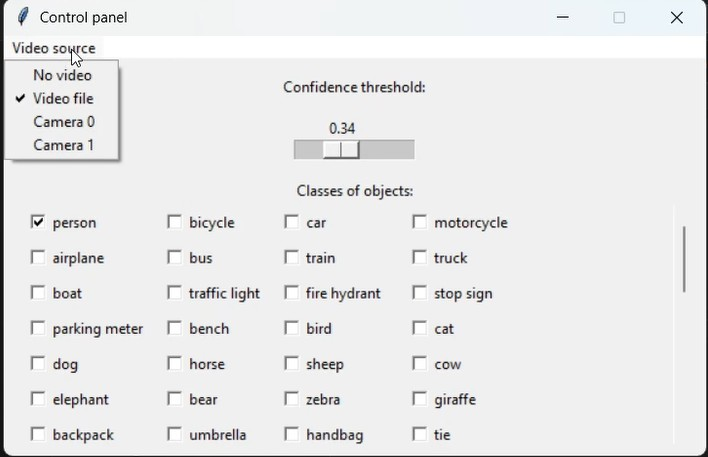
\includegraphics[width=0.79\linewidth]{r_implementacja/panel_sterowania/panel.jpg}
    \caption{Panel sterowania graficznego interfejsu użytkownika.}
    \label{fig:panel-sterowania}
\end{figure}

Zmiana parametrów detektora może odbywać się w trakcie działania zadań dektecji obiektów. Po wystąpieniu wydarzania nowe wartości parametrów nadpisują ustawienia detektora i od tego momentu tryb inferencji będzie korzystać z nowych parametrów.

Wybranie źródła wideo skutkuje uruchomieniem ustalonej sekwencji funkcji logicznych. Sekwencja ta objemuję następujące kroki:
\begin{enumerate}
    \item Pobranie klatki obrazu z wybranego źródła wideo.
    \item Detekcja ustawionych klas obiektów na bazie pobranej klatki.
    \item Jeżeli wykryto choć jeden obiekt:
    \begin{enumerate}
        \item Przetworzenie klatki w celu narysowania wygenerowanych prostokątów ograniczających. 
        \item Alarmowanie w formie dźwiękowej. 
    \end{enumerate}
    \item Dostarczenie klatki do bufora.
    \item Pobranie klatki z bufora oraz wyświetlenie jej w wyświetlaczu GUI.
\end{enumerate} 
Sekwencja jest powtarzana do momentu zakończenia się pliku wideo lub wyłączenia bądź zmiany źródła wideo. 

Na podstawie funkcji systemu zobrazowano przykładowy scenariusz wykorzystania systemu przez użytkownika z kolejnymi krokami na ryskunkach \ref{fig:mockup-1}, \ref{fig:mockup-2}, \ref{fig:mockup-3}, \ref{fig:mockup-4}. Przykładowe użycie to nagranie sceny ze znajdującym się człowiekiem (twarz zamazano).


\begin{figure}[H]
    \centering
    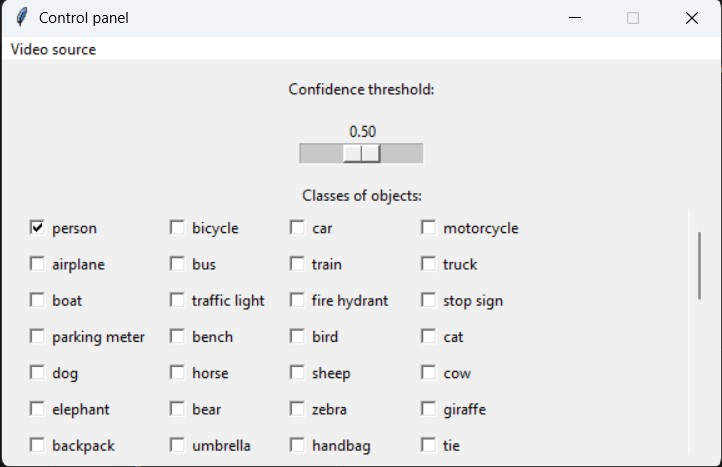
\includegraphics[width=\linewidth]{r_implementacja/panel_sterowania/panel_mockup.jpg}
    \caption{GUI w chwili uruchomienia aplikacji. Domyślne paramtry detektora to próg ufności równy 0.5 oraz klasa \emph{człowiek} jako zbiór wykrywanych klas.}
    \label{fig:mockup-1}
\end{figure}

\begin{figure}[H]
    \centering
    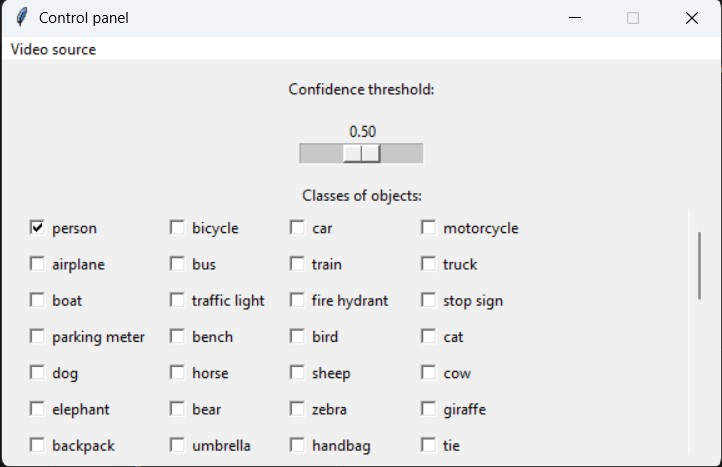
\includegraphics[width=\linewidth]{r_implementacja/panel_sterowania/panel_mockup.jpg}
    \caption{GUI w chwili uruchomienia aplikacji. Domyślne paramtry detektora to próg ufności równy 0.5 oraz klasa \emph{człowiek} jako zbiór wykrywanych klas.}
    \label{fig:mockup-2}
\end{figure}

\begin{figure}[H]
    \centering
    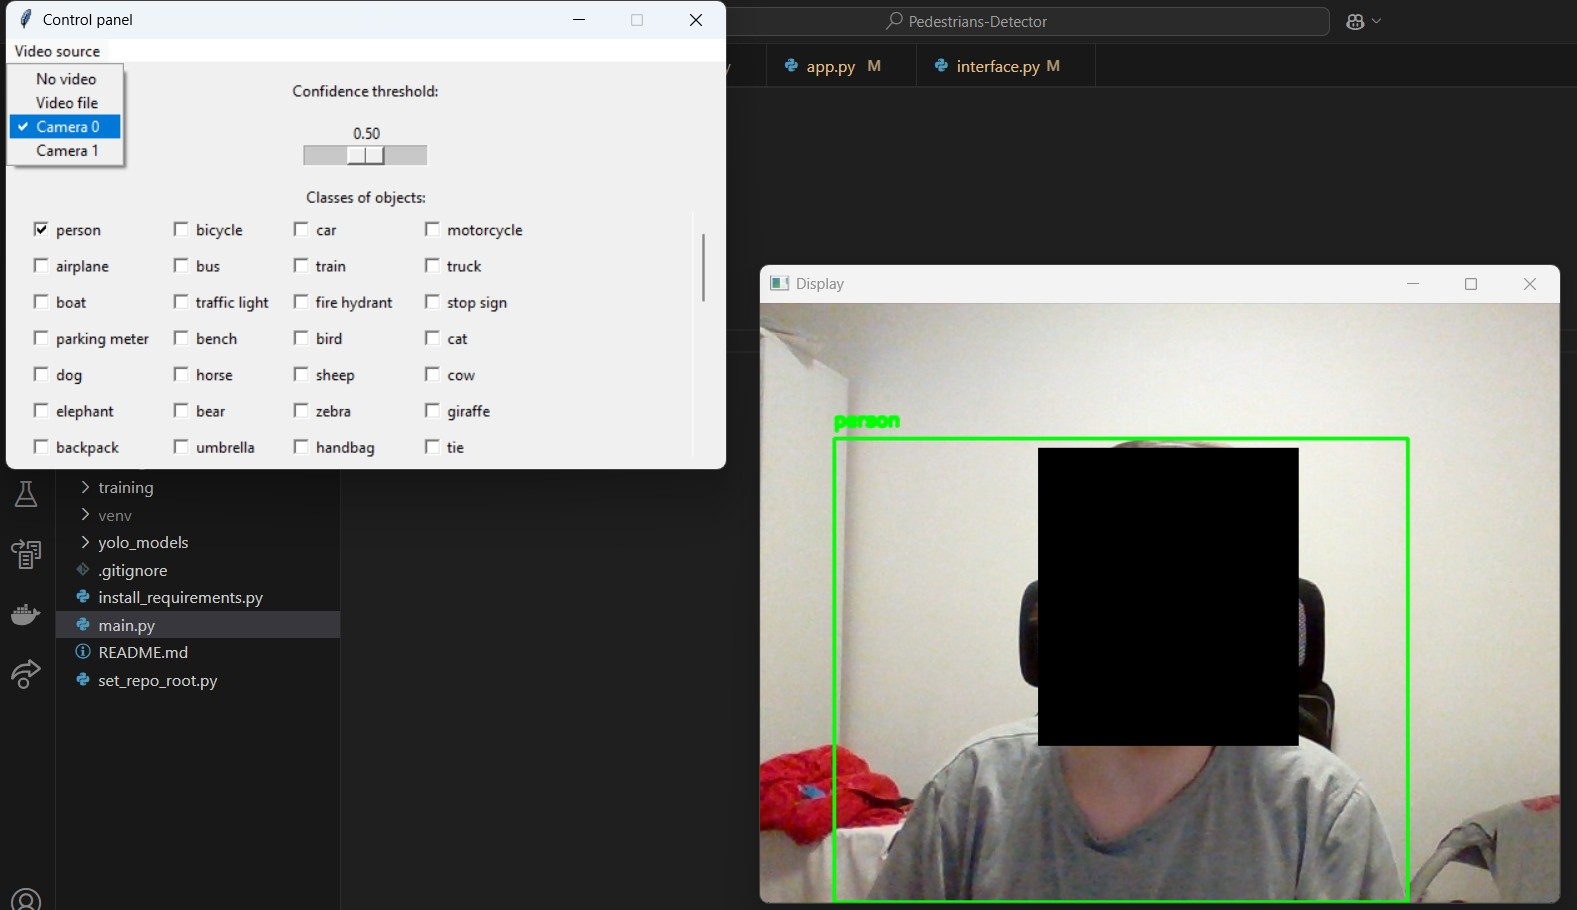
\includegraphics[width=\linewidth]{r_implementacja/panel_sterowania/camera_50.jpg}
    \caption{Uruchomienie wyświetlacza dla domyślncyh parametrów detektora oraz kamery o indeksie 0.}
    \label{fig:mockup-3}
\end{figure}

\begin{figure}[H]
    \centering
    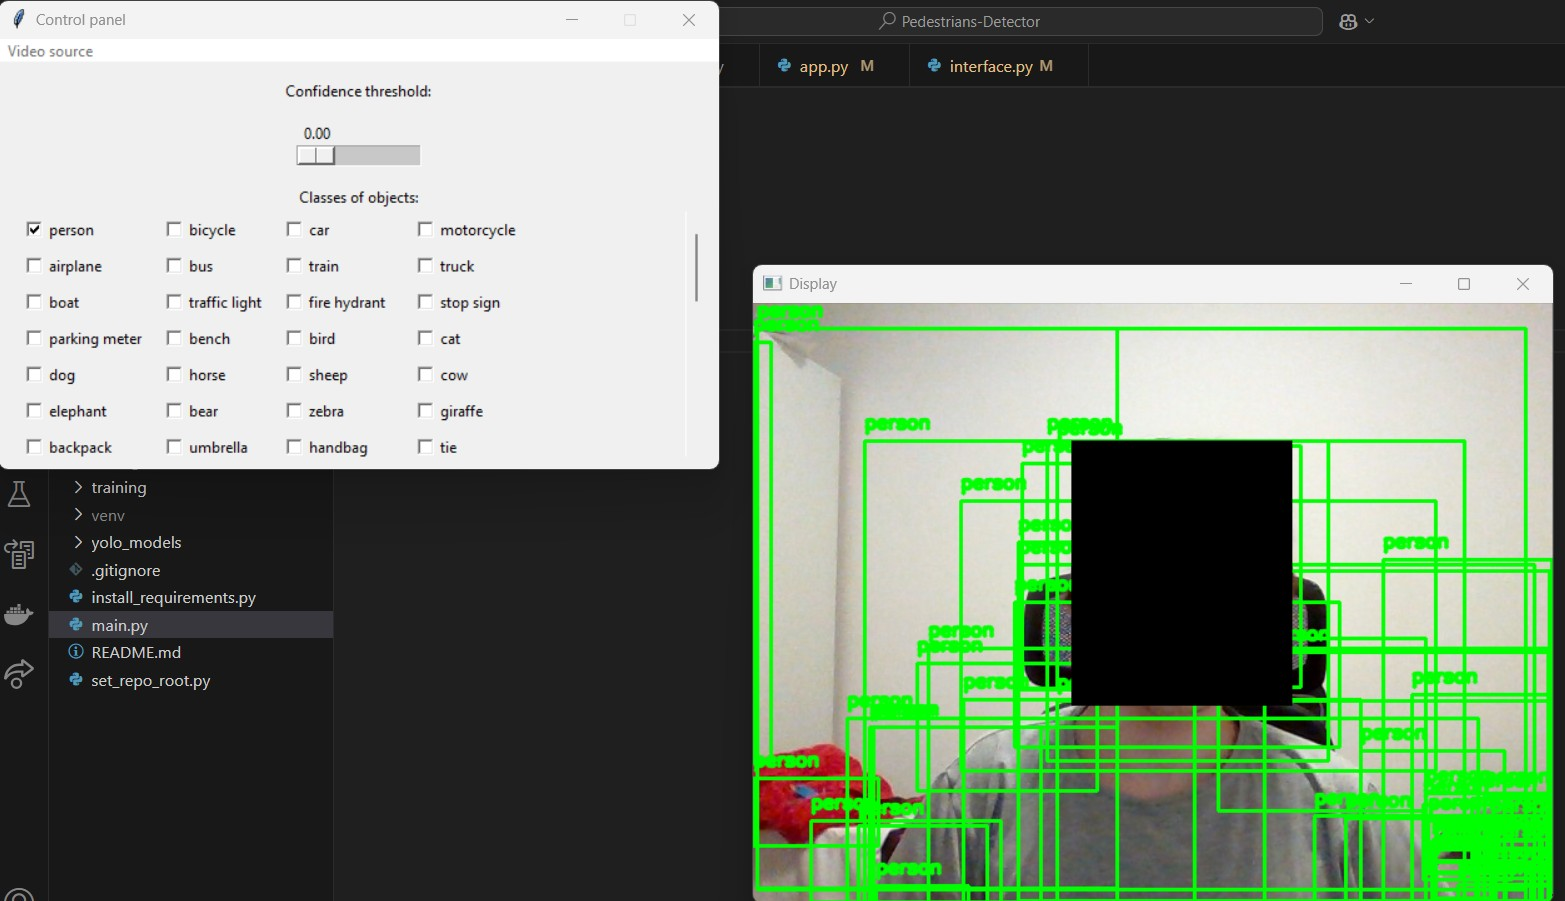
\includegraphics[width=\linewidth]{r_implementacja/panel_sterowania/camera_0.jpg}
    \caption{Zmiana progu ufności na 0.00.}
    \label{fig:mockup-4}
\end{figure}

\begin{figure}[H]
    \centering
    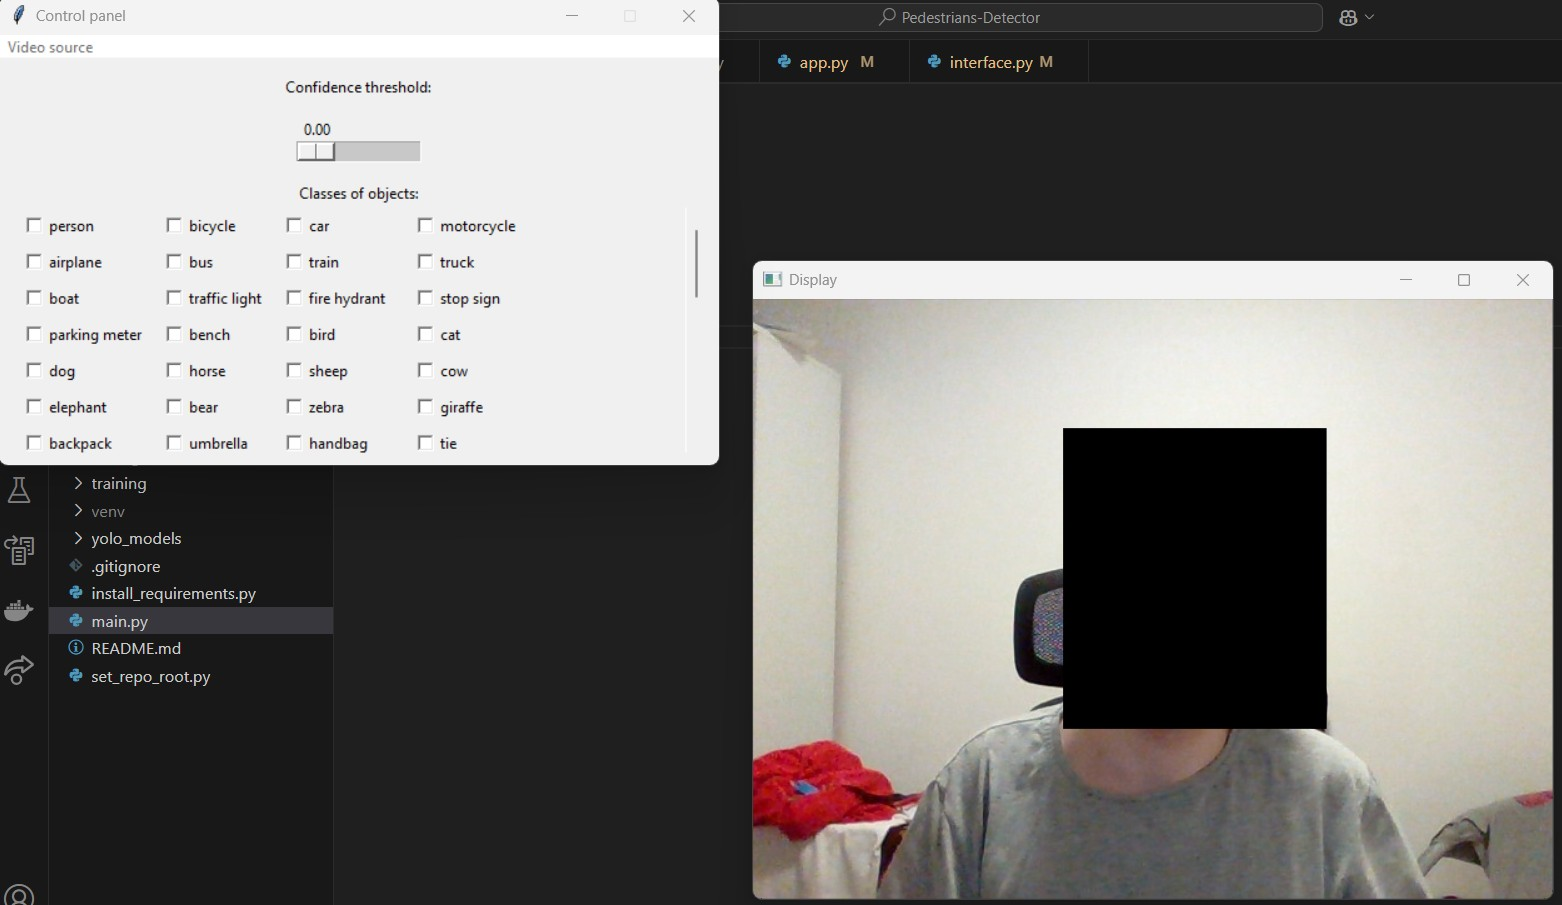
\includegraphics[width=\linewidth]{r_implementacja/panel_sterowania/camera_no_person.jpg}
    \caption{Usunięcie klasy człowiek z wykrywanych obiektów.}
    \label{fig:mockup-5}
\end{figure}


\section{Architektura systemu na poziomie klas}
Oprogramowanie podzielono na sześć klas: \emph{App}, \emph{VideoCapture}, \emph{YoloInferenceConfig}, \emph{ImageProcessor}, \emph{VideoProcessingEngine} oraz \emph{GUI}.

\emph{App} jest punktem centralnym aplikacji. W tym miejscu rozpoczyna się program i tworzone są instancję pozostałych pięciu klas. Pierwszym zadaniem klasy jest uruchomienie wszystkich modułów w odpowiedniej kolejności. Następnie klasa ta służy jako interfejs do komunikacji między sekcją interfejsu graficznego (\emph{GUI}), a sekcją logiczną -- w tym do pobrania informacji o dostępnych kamerach (\emph{VideoCapture}), ustawienia danych detektora (\emph{ImageProcessor}) oraz obustronnej komunikacji z silnikiem przetwarzającym klatki wideo (\emph{VideoProcessingEngine}). 
Ponadto, klasa ta implementuje metodę, która uruchamia alarm dźwiękowy (\emph{{play\_audio\_alert}}). 

\emph{VideoCapture} służy do obługi źródła wideo. Klasa dostarcza kluczową metode, \emph{get\_frame}, której wywołanie zwraca informację o tym czy źródło wideo nadal jest dostępne oraz najnowszą dostępną klatkę z kamery. Ponadto warto wyróżnić metodę do pozyskania dostępnych do użycia kamer (\emph{get\_available\_sources}).

\emph{YoloInferenceConfig} jest to klasa, której głównym celem jest przechowywanie parametrów inferencji (progu ufności oraz wykrywanych klas) oraz dostarczenie metod do zmiany tych parametrów. Klase utworzono dla zachowania większej czytelności kodu w \emph{ImageProcessor}, dlatego też jest ona dziedziczona przez \emph{ImageProcessor} właśnie. W chwili uruchomienia aplikacji, klasa jest inicjalizowana domyślnymi parametrami: próg ufności równy $0.5$ oraz \emph{człowiek} jako wykrywany klasa. 

\emph{ImageProcessor} służy do manipulacji oraz analizy obrazu. Kluczowe dwie metody to \emph{detect\_objects}, zwracająca liczbe wykrytych obiektów oraz wyniki detekcji na podstawie podanej klatki obrazu, oraz \emph{visualize\_objects\_presence}, która na postawie w.w. wyników detekcji, rysuję prostokąty ograniczające dookoła wykrytych obiektów.

\emph{VideoProcessingEngine} stworzono w celu koordynacji i rozplanowania wszystkich zadań koniecznych do uzyskania kolejnych klatek obrazu, gotowych do wyświetlenia w graficzym interfejsie użytkownika, oraz realizacji celu alarmowania dźwiękowego użytkownika, kiedy jest to konieczne. Zbiór zadań zawiera pobranie klatki z kamery, detekcję obiektów, przetworzenie klatki w celu wizualizacji obiektów, alarmowanie dźwiękowe użytkownika oraz umieszczenie klatki w buforze wyjściowym. Zadania te nie mają implementacji w samej klasie i są metodami wywoływanymi z innych klas (\emph{App}, \emph{ImageProcessor} oraz \emph{VideoCapture}). Jest to najważniejszy element całego systemu, określający w stopniu znacznym jego architekturę, scalającym kluczowe komponenty oraz mającym główny wpływ na wydajność rozwiązania.

\emph{GUI} to graficzny interfejs użytkownika naszej aplikacji. Składa się on z wyświetlacza klatek obrazu oraz panelu sterowania. Tak jak to wcześniej wspomniano, używa on \emph{App} w celu komunikacji z resztą modułów. Tyczy się to zarówno komunikacji dwustronnej z \emph{ImageProcessor} oraz \emph{VideoCapture}, potrzebnej do panelu sterowania, oraz jednostronnej z \emph{VideoProcessingEngine} w celu pobrania klatki bufora wyjściowego.  

Opisane zależności komunikacyjne między klasami oraz programowe zrealizowanie tej komunikacji zilustrowano uprosczonym diagramem UML na rysunku \ref{fig:uprosczony-diagram-klas}. Pełen diagram UML przedstawiono na rysunku \ref{fig:diagram-klas}. 

\begin{figure}[H]
    \centering
    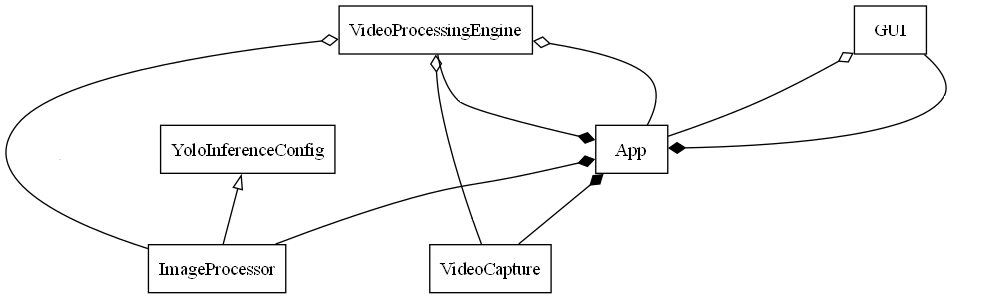
\includegraphics[width=\linewidth]{r_implementacja/klasy/simplified_classes.png}
    \caption{Uprosczony diagram klas UML (bez metod i pól) wygenerowany przez bilbiotekę \emph{pylint}.}
    \label{fig:uprosczony-diagram-klas}
\end{figure}


\begin{figure}[H]
    \centering
    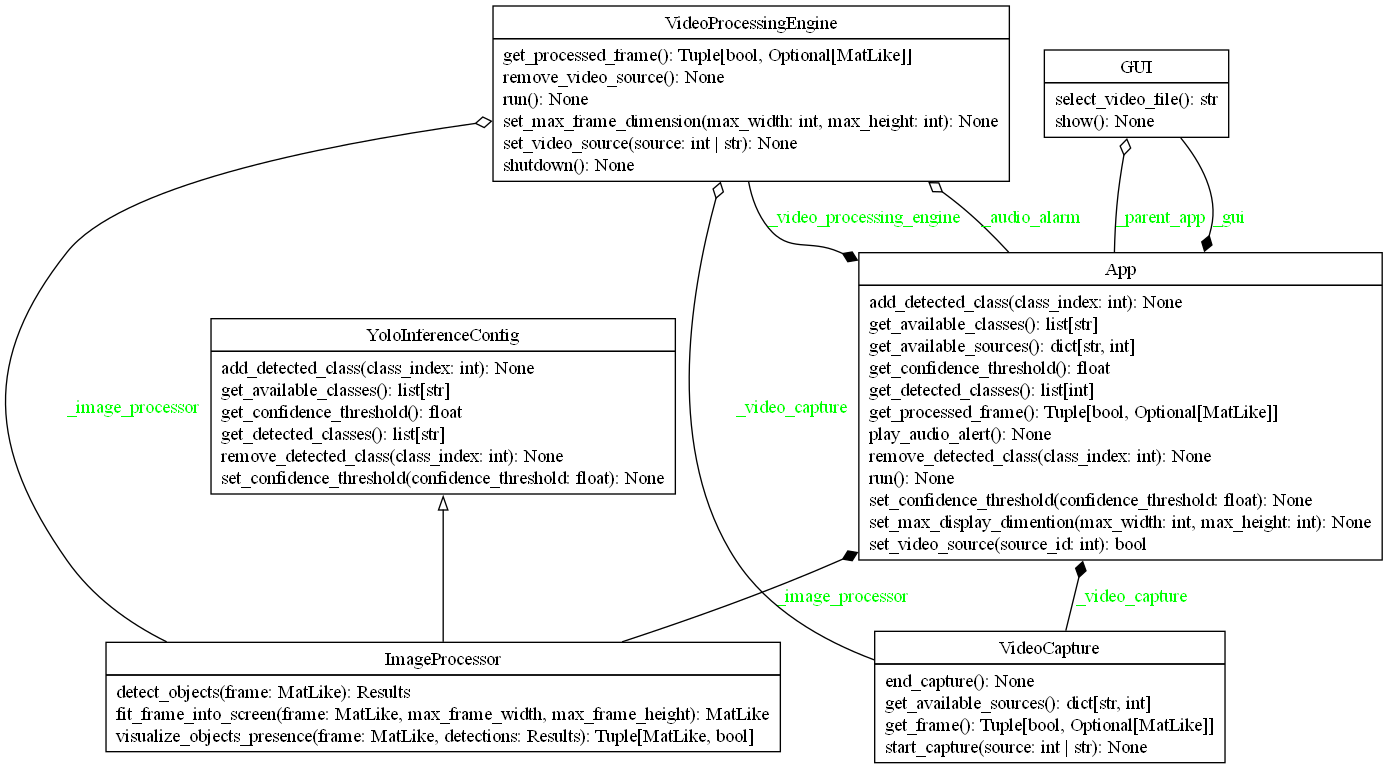
\includegraphics[angle=270, scale = 0.5]{r_implementacja/klasy/classes_MyProject.png}
    \caption{Diagram klas UML wygenerowany przez bilbiotekę \emph{pylint}.}
    \label{fig:diagram-klas}
\end{figure}


\section{Szczegóły implementacyjne i decyzje architektoniczne}
W sekcji tej opisano zastosowane wielowątkowe podejście architektoniczne. Przedstawiono argumenty za wybraniem tego typu architektury oraz rozwiązanie problemów przez nią generowanych. 

Z perspektywy programistycznej, jedną z pierwszych iteracji oprogramowania był system oparty na architekturze jednowątkowej. Klasa \emph{VideoProcessingEngine} przy użyciu nieskończonej pętli, w sposób sekwencyjny wywoływała kolejne metody: pobór klatki z kamery, detekcja obiektów, alarmowanie dźwiękowe, wizualizacja obiektów oraz umieszczenie klatki wynikowej w buforze wyjściowym. W celu pobrania klatki z bufora wyjściowego, klasa \emph{GUI} periodycznie wywoływała do tego odpowiednią metodę. Warto rozjaśnić, iż mimo użycia bufora, aplikacja działała w sposób sekwencyjny, ponieważ wbudowana w tkinter funkcja \emph{after} określała czas, po którym zaplanowano wykonananie przekazana do niej metody w ramach wspólnego wątku głownego. Realizacja periodyczna została zaimplementowana poprzez wywołanie metody \emph{\_update\_frame}, która w pewnym fragmencie swojego kodu wyołuje siebie samą poprzez funkcję \emph{after} (\ref{lst:tkinter-after-function}). Przykład użycia tego mechanizmu zaprezentowany jest w listingu \ref{lst:tkinter-after-function}.

\begin{lstlisting}[caption={Fragment kodu zawierający użycie mechanizmu \emph{after}}, label={lst:tkinter-after-function}]
AFTER_DELAY = 1 # Opoznienie w milisekundach
class GUI:
    # Metoda rozpoczynajaca wyswietlanie klatek:
    def _start_displaying(self) -> None:
            self._is_displaying = True
            cv.namedWindow('Display', cv.WINDOW_NORMAL)
            cv.moveWindow('Display', 0, 0)
            # Wywolanie metody:
            self._update_frame()

    # Metoda pobierajaca klatke z bufora, a nastepnie ja wyswietlajaca
    def _update_frame(self) -> None:
        if not self._is_displaying:
            self._stop_displaying()
            return

        # Pobranie klatki z bufora:
        is_capture_on, frame = self._frame_generator.get_processed_frame()

        if is_capture_on:
            if frame is not None:
                self._show_frame(frame)
            # Kolejne wywolanie _update_frame funkcja after.
            # Wywolanie nastapi po "AFTER_DELAY" milisekundach.
            # Uzycie after powoduje nieskonczone wywolanie _update_frame do momentu zakonczenia wyswietlania.
            # Uzycie after pozwala kazdemu wywowaniu _update_frame na zakonczenie sie i zwolnieniu pamieci. 
            self._root.after(AFTER_DELAY, self._update_frame)
        else:
            self._frame_generator.set_video_source(NO_VIDEO)
            self._selected_video_source_id.set(NO_VIDEO)
                self._stop_displaying()
\end{lstlisting}

Synchronizacja GUI oraz wykonywanie czasochłonnych operacji m.in. detekcji obiektów w tym samym wątku czyniło tę iterację wolną, a także nieresponsywną. Podjętą próbą optymalizacji było przeniesienie wykonania detekcji obiektów z CPU na GPU umożliwione dzięki interfejsowi programistycznemu do YOLOv8n (opis użytego parametru w rodziale \ref{chap:wprowadzenie-yolo_interjes}). Zmiana ta znacznie poprawiła wydajność i pozostała ona aż do ukończonej wersji systemu. Mimo wszystko zmiana ta nie była wystarczająca. Dlatego też zdecydowano się zastosować architekturę wielowątkową. 

Pierwszym problemem jaki napotkano były ograniczenia  GUI w środowisku wielowątkowym. tkinter, jak większość dostępnych rozwiązań interjesu graficznego, jest zaprojektowany do użycia w ramach wątku głównego aplikacji. Integracja z dodatkowymi wątkami może powodować niezdefiniowane zachowania. Dlatego też zrezygnowano z pomysłu wyświetlania klatki w ramach wątku przetwarzającego obraz zaraz po otrzymaniu takiej klatki, co zmusiło do pozostania przy mechanizmie bufora wyjściowego. 

